\documentclass[convert={density=300,outext=.png}]{standalone}
\usepackage{tikz}
\begin{document}
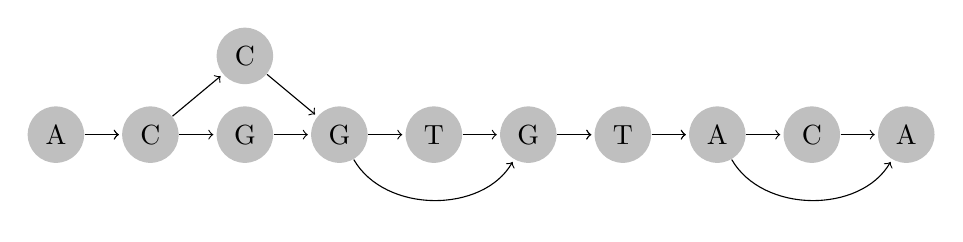
\begin{tikzpicture}[shorten >=1pt,->]
  \def\f{1.2};
  \def\fy{1}

\tikzstyle{vertex}=[circle,fill=black!25,minimum size=17*\f pt,inner sep=0pt]
\node[vertex][] (P1) at (0*\f,0) {A};
\node[vertex][] (P2) at (1*\f,0) {C};
\draw (P1) -- (P2);
\draw (P1) -- (P2);
\node[vertex][] (P3) at (2*\f,0) {G};
\draw (P2) -- (P3);
\node[vertex][] (P4) at (2*\f,1) {C};
\draw (P2) -- (P4);
\node[vertex][] (P5) at (3*\f,0) {G};
\draw (P3) -- (P5);
\draw (P4) -- (P5);
\node[vertex][] (P6) at (4*\f,0) {T};
\draw (P5) -- (P6);
\node[vertex][] (P7) at (5*\f,0) {G};
\draw (P6) -- (P7);
\path [->] (P5) edge[bend right=60] node {} (P7);
\node[vertex][] (P8) at (6*\f,0) {T};
\draw (P7) -- (P8);
\draw (P7) -- (P8);
\node[vertex][] (P9) at (7*\f,0) {A};
\draw (P8) -- (P9);
\draw (P8) -- (P9);
\node[vertex][] (P10) at (8*\f,0) {C};
\draw (P9) -- (P10);
\node[vertex][] (P11) at (9*\f,0) {A};
\draw (P10) -- (P11);
\path [->] (P9) edge[bend right=60] node {} (P11);
\end{tikzpicture}
\end{document}
